%% galaxies.tex

Weighing galaxies is not easy, partially because most of their components are
invisible, dark matter being the most elusive amongst them.  However, much like
tree branches move in the wind, orbits of stars still feel the gravitational
pull from the mass inside them.  Stars in a more massive galaxy will move with
higher orbital speeds than in lower-mass galaxies; more formally, the mass $M$
inside the (circular) orbit of radius $r$ is $M(<r) \propto V^{2}r$, where $V$
is the orbital speed of the star.  Accordingly, by measuring the velocities of
stars at a particular distance from the centre, a mass estimate for the galaxy
can be calculated, which is a simple application of Newton's first law combined
with Kepler's law.  It is equivalent to assuming the galaxy is in hydrostatic
equilibrium formulated by the virial theorem 
\begin{equation}
    \begin{aligned}
        &V^{2} = \frac{GM(<r)}{r}\\
        &2E = -U,
    \end{aligned}
\end{equation}
where $E$ and $U$ are the kinetic and potential energy respectively
\sidecite{BinneyTremaine08, Zwicky1933}.  When the individual orbits of stars
cannot be resolved in {e.g.} spiral galaxies, other 'tracers' can be used such
as atomic hydrogen gas measured through 21-cm line radiation in the radio
spectrum \sidecite{vandeHulst1951, Muller1951, vandeHulst1954}, or as
perturbations in the optical wavelengths.  For ellipticals, the velocity
dispersion $\sigma$ measured by the spread of spectral absorption lines is the
observable which analogously measures their mass as $M(<r) \propto \sigma^{2}r$
\sidecite{Davies83, Schechter80, Wang20}.  The observables measured are, in most
cases, treated as dynamical equilibria, or temporal averages and therefore yield
(by implicitly assuming the ergodic theorem) 1-dimensional (1D) models such as
the rotation curve $V(r)$ \sidecite{Bosma17, MartinezMedina20, Ablimit20,
Cautun20, Bovy12}.

The endeavour of measuring velocities was and still is complicated, even within
the Milky Way.  Earth is revolving around our Sun, and the Solar System is
orbiting around the Galactic centre, which means relative motions have to be
carefully examined.  From some locations on Earth, a dense strip of starlight is
visible across the night sky which is indicative of the Galaxy's disk structure.

\begin{figure}[h]
    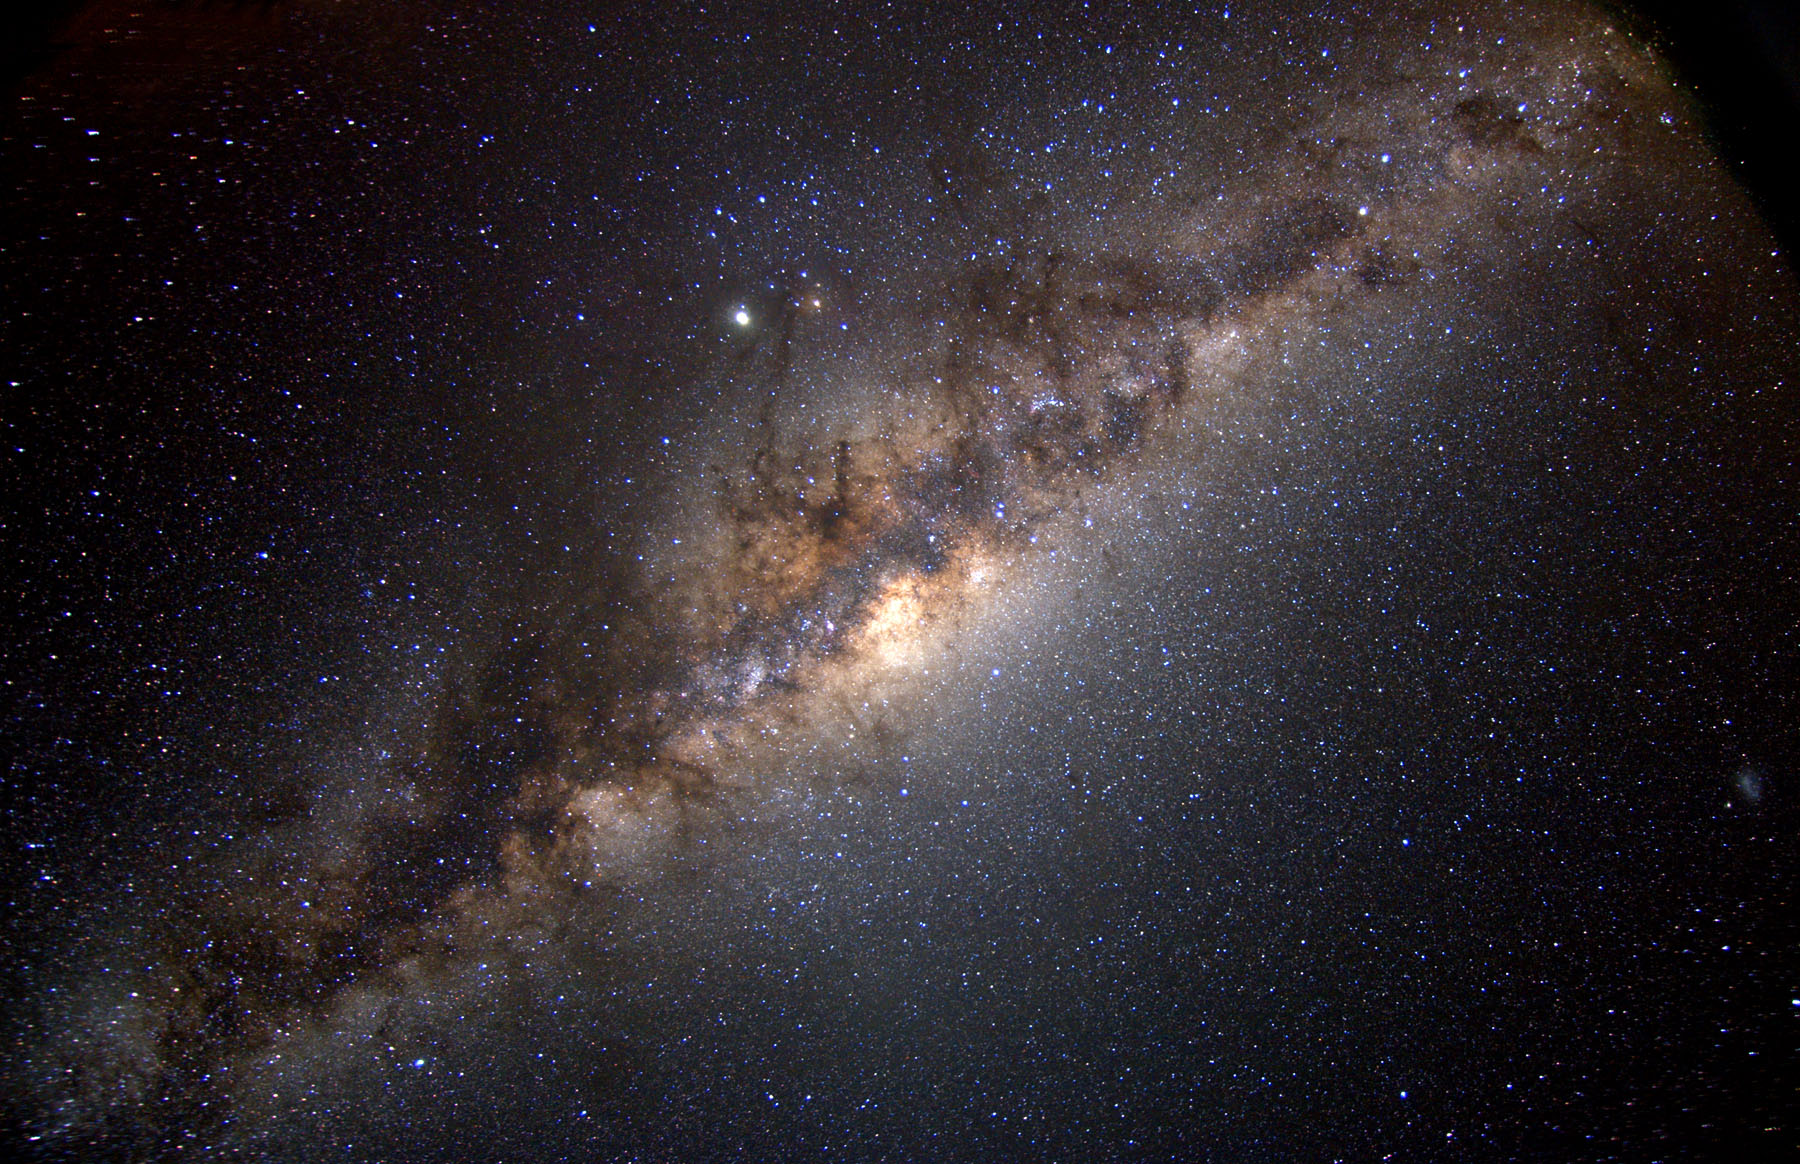
\includegraphics{apod080104}
    \caption[The Milky Way: APOD 2008 January
    4]{\href{https://apod.nasa.gov/apod/ap080104.html}{APOD 2008 January 4}: The
    Milky Way at 5000 meters.\\
    View on our own galaxy from within (recorded in the Chilean Andes).  The
    band of the dense collection of stars from the disk and the Galactic centre
    is partially covered by the typical extinction features due to dust
    clouds.  It indicates that the Milky Way possesses a stellar disk.\\
    \textit{Credit \& Copyright: Serge Brunier}}
    \figlbl{milkyway}
\end{figure}

From far away it is quite easy to recognise the typical morphology of other
galaxies through direct observations\sidenote{Provided the telescope has enough
angular resolution.}.  Measuring their rotational properties already becomes
increasingly difficult, deducing the shape and rotation patterns of the Milky
Way from within however is an undertaking of its own.

A seemingly random and dense distribution of stars as it appears in galaxies
should in principle collapse towards its potential well.  Like in many other
astrophysical scenarios, pressure gradients can take a stabilising role and
balance gravity.  These balancing pressures depend on different physical
processes and generally define limiting scales.  For some galaxies, e.g.
ellipticals, the stars' random motions are the dominant drivers towards
stability, for spiral galaxies it is their rotation about the disk's centre.  In
contrast to orbiting systems such as the Sun and Earth, where most of the mass
is located near the guiding centre of the orbits, the Milky Way's mass
distribution is more complex with different elements such as various forms of
hydrogen gas, dust, stars, and stellar remnants.  In general, the study of
galactic rotation through stars can yield insights not only into the galaxy's
morphology, but also into its formation history and mass composition.  

A powerful tool for this is the rotation curve $V(r)$.  It characterises the
orbital velocity as a function of distance from the Galactic centre. By
measuring how $V(r)$ behaves with radius, we can draw conclusions about the
Milky Way's size, total mass, and the distribution thereof.  A solid-body
rotation $V \propto r$ would mean that the enclosed mass ideally increases with
$r^{2}$, Keplerian orbits go as $V \propto r^{-\half}$, whereas $V \propto
\text{const.}$ is a result of the enclosed mass increasing as $r$.

Milky Way's rotation curve can be probed through its stars. Prime observable is
the radial velocity $v_{z}$, and in principle the tangential velocity $v_{t}$,
distance from Earth $d$ and longitude on the sky $l$ too.  Measurements of these
quantities can be combined to the so-called \textit{Oort's constants}
%
\begin{equation}\eqlbl{obs_oortsC}%
    \begin{aligned}%
        &A = \frac{v_{z}}{d\sin{2l}} \\
        &B = \frac{v_{t}}{d} - A\cos{2l}.
    \end{aligned}%
\end{equation}%
%
A caveat is the assumption that the stars, including the Sun, are on circular
orbits, which is only approximately true.  Moreover, it assumes the Milky Way
has a monotonically decreasing, symmetric potential.  Again, this is not
entirely true as spiral arms can introduce over-densities which manifest as
asymmetries and locally break monotonic behaviour in the potential.  Still,
within their limits the Oort's constants are very useful, because they can be
rewritten as
%
\begin{equation}\eqlbl{oortsC}
    \begin{aligned}%
        &A = -\frac{1}{2} \left[\frac{\derivd V}{\derivd r} - \frac{V_{0}}{R_{0}}\right] \\
        &B = -\frac{1}{2}\left[\frac{V_{0}}{R_{0}} + \frac{\derivd V}{\derivd r}\right].
    \end{aligned}%
\end{equation}
%
Recent measurements from the Gaia survey determined these constants with
$A=15.3\pm0.4\,\Oortsunitsalt$ and $B=-11.9\pm0.4\,\Oortsunitsalt$
\sidecite{Bovy17}.  These constants express the shear and vorticity of the disk
in the solar neighbourhood.  The shear essentially measures a deviation from
solid-body rotation, the vorticity how the angular momentum varies with small
changes in radius.  Adding both $A+B = -\frac{\derivd V}{\derivd r}$ yields the
velocity gradient, which seems to be relatively flat with $3.4\;\Oortsunitsalt$
as was expected from previous and alternative investigations.  From the velocity
gradient the mass density for the Milky Way can be written as follows (see
\sideciteay{BinneyTremaine08})
%
\begin{equation}\eqlbl{MWrho}
    \begin{aligned}
        \rho_{MW} &\quad\sim\quad \frac{(A+B)^2}{2\pi} \\
                  &\quad\sim\quad 2 \times 10^{-33}\;\sec^{-2}
    \end{aligned}
\end{equation}
%
As a rough estimate, this is of the order of the mean density of the Milky Way
within its volume, as long as the assumptions of the Oort's constants are valid.
This is obviously not the case outside the edge of the Galaxy. However, the size
of the Milky Way is not clearly known.  The issue lies in the ambiguity
regarding the definition of the edge of the Galaxy.  In the literature the
'$R_{200}$' is frequently used, sometimes also called the 'virial' radius within
which the mean density equals 200 times the cosmological critical density.
Another less back-of-the-envelope definition is the 'splashback' radius, a
caustic manifested in a drop in density or radial velocity.  At roughly half the
splashback radius an edge can be defined where virialized material has completed
at least two pericentric passages.  This radius was recently determined for the
Milky Way to be $R_{MW} \sim 290\;\mathrm{kpc}$ \sidecite{Deason20}, and seems
to define an edge where our assumptions should still hold.  Within a cubic
megaparsec the Milky Way's mean density in \eqref{MWrho} should therefore be
diluted by the corresponding volume factor $(R_{MW} / \mathrm{Mpc})^{3} \sim 2
\times 10^{-2}$, yielding

\begin{equation}\eqlbl{MWperMpc}
    \frac{M_{MW}}{\mathrm{Mpc}^{3}} \quad\sim\quad 4 \times 10^{-35}\;\sec^{-2}
\end{equation}

%%%%%%%%%%%%%%%%%%%%%%%%%%%%%%%%%%%%%%%%%%%%%%%%%%%%%%%%%%%%%%%%%%%%%%%%%%%%%%%%	
\par\noindent\rule{\textwidth}{0.8pt}

Comparing this quantity to the cosmological matter density, which is roughly
30\% of the total energy content in the Universe.

\begin{equation}
    \begin{aligned}
        \rho_{m} &=\quad 0.3\cdot\frac{3}{8\pi}\Ho^{2} \\
                 &\sim\quad 2 \times 10^{-37}\;\sec^{-2}
    \end{aligned}
\end{equation}

Comparing these two quantities yields the percentage of Milky-Way-like galaxies
per cubic megaparsec
\begin{equation}
    \frac{\rho_m}{M_{MW}/\mathrm{Mpc}^{3}} \sim 0.5\%.
\end{equation}

In $(1\;\mathrm{Gpc})^{3}$ roughly $10^7$ MW

$10^{-3}$ of sources are strongly lensed